% \documentclass[aip,jcp,preprint,unsortedaddress,a4paper,onecolum]{revtex4-1}
\documentclass[aip,jcp,a4paper,reprint,onecolumn]{revtex4-1}
% \documentclass[aps,pre,twocolumn]{revtex4-1}
% \documentclass[aps,jcp,groupedaddress,twocolumn,unsortedaddress]{revtex4}

\usepackage[fleqn]{amsmath}
\usepackage{amssymb}
\usepackage[dvips]{graphicx}
\usepackage{color}
\usepackage{tabularx}
\usepackage{algorithm}
\usepackage{algorithmic}
\newcommand{\diag}{\textrm{diag}}

\makeatletter
\makeatother

\begin{document}

\noindent
In the PRE paper, we consider the mode of the velocity
\begin{align}
  \hat v(k) = \sum_{i=1}^N v_i \sin(k z_i),
\end{align}
which is an approximation to the Fourier tranform of the velocity profile $v(z)$, i.e.
\begin{align}
  \hat v(k) = \int_{-\infty}^{+\infty} v(z) \sin(kz) dz
\end{align}
and we have
\begin{align}\label{eqn:tmp3}
  v(z) = \frac1{2\pi}\int_{-\infty}^{+\infty} \hat v(k)\sin(kz) dk
\end{align}\\
% where $v(z)$ is defined to be
% \begin{align}
%   v(z) = \sum_{i=1}^N v_i \delta (z - z_i).
% \end{align}

\noindent
Instead of the full fluid region, we now consider a ``window'' of the fluid region saying
$\Omega_w = [-h_w, h_w]$.
We assume that the density of the fluid in the window is roughly constant.
Now we compute the ``mode''
\begin{align}
  \hat v_w(k) = \sum_{i\in\Omega_w} v_i \sin(k z_i),
\end{align}
It is actually the approximation to the integral
\begin{align}\label{eqn:tmp5}
  \hat v_w(k) = \int_{-h_w}^{h_w} v(z) \sin(kz) dz
\end{align}
Insert Eq.~\eqref{eqn:tmp3} into \eqref{eqn:tmp5}, we have
\begin{align}
  \hat v_w(k) = \frac{1}{2\pi}\int_{-\infty}^{+\infty} d\xi \,\hat v(\xi) \int_{-h_w}^{h_w}dz  \sin(kz) \sin(\xi z)
\end{align}
In the discretized form, we solve the linear system:
\begin{align}\label{eqn:tmp7}
  \Delta \xi\sum_j A_{ij} \hat v_j = (\hat v_w)_i, \quad i,j = 1, \cdots, K
\end{align}
where
\begin{align}
  A_{ij} = \frac{1}{2\pi} \int_{-h_w}^{h_w}dz  \sin(k_i z) \sin(\xi_j z), \quad (\hat v_w)_i,  = \hat v_w(k_i), \quad \hat v_j  =  \hat v(\xi_j) 
\end{align}
and $K$ is the number of modes we want to investigate.
\\
% When $h_w$ goes to infinity, the $A_{ij}$ is diagonal, so we get back to the PRE case.

\noindent
Now we discard the constant $\Delta \xi$ on the RHS of \eqref{eqn:tmp7}, because in the end we compute the normalized $\hat v$ autocorrelation.
Eq.~\eqref{eqn:tmp7} becomes a linear system
\begin{align}\label{eqn:tmp9}
  A \hat v = \hat v_w
\end{align}
The matrix $A$ is symmetric and positive definite, therefore we have the eigen value decomposition of $A$:
\begin{align}
  A = T \Lambda T^\top
\end{align}
where $\Lambda = \diag\{ \lambda_1, \cdots \lambda_K\}$ is a diagonal matrix,
and the diagonal elements are eigenvalue sorted in descending order:
$\lambda_1 \leq \lambda_2 \leq, \cdots, \leq \lambda_K$.
The matrix $T$ is column-wisly composed by eigenvectors of $A$, i.e.~$A = [t_1, \cdots, t_K]$,
where $t_i$ (size $K\times 1$) is the $i$-th eigenvector corresponding to eigenvalue $\lambda_i$.
By this decomposition, Eq.~\eqref{eqn:tmp9} is solved by
\begin{align}
  \hat v = T \Lambda^{-1} T^\top \hat v_w
\end{align}
where $T^\top \hat v_w$ is the projection to the $A$'s eigenspace, and $T$ transform the vector $\Lambda^{-1} T^\top \hat v_w$ back to  k-space.
\\

\noindent
It should be noted that when $k$ takes a range of values with uniform interval, for example $[0.5 : 0.01: 3.0]$,
there are only few eigenvalue of $A$ are siginificant. For example, in the small system who has a channel width of roughly 4.6~nm,
when $h_w = 4.6$~nm, and $k$ takes the above range, the leading eigenvalues of $A$ are
\begin{align}
  314.1,\ 313.6,\ 289.8,\ 175.3,\ 62.4,\ 1.5,\ 1.2\times10^{-2}, 3.5\times 10^{-5}, \cdots
\end{align}
Therefore, there are roughly 5 eigenvalues are siginificant. We denote the number of significant eigenvalues to be $M$.
$\tilde T = [t_1, \cdots, t_M]$ is the matrix composed by siginificant eigenvectors, and
$\tilde \Lambda = [\lambda_1, \cdots, \lambda_M]$ is the diagonal matrix of siginificant eigenvalues.
Eq.~\eqref{eqn:tmp9} is solved by revised formula:
\begin{align}\label{eqn:solver}
  \hat v = \tilde T \tilde\Lambda^{-1} \tilde T^\top \hat v_w
\end{align}


\noindent
By using the formula \eqref{eqn:solver}, given $h_w$ and $k$ range,
we compute $\hat v$, and then estimate the characteristic decaying time from the autocorrelation of $\hat v_i = \hat v(k_i)$.
A preliminary result is given in Fig.~\ref{fig:tmp1}. The intrisic mode and the corresponding decay time is robust w.r.t the choice of eigenvalues ``cut-off'' $M$.
\begin{figure}
  \centering
  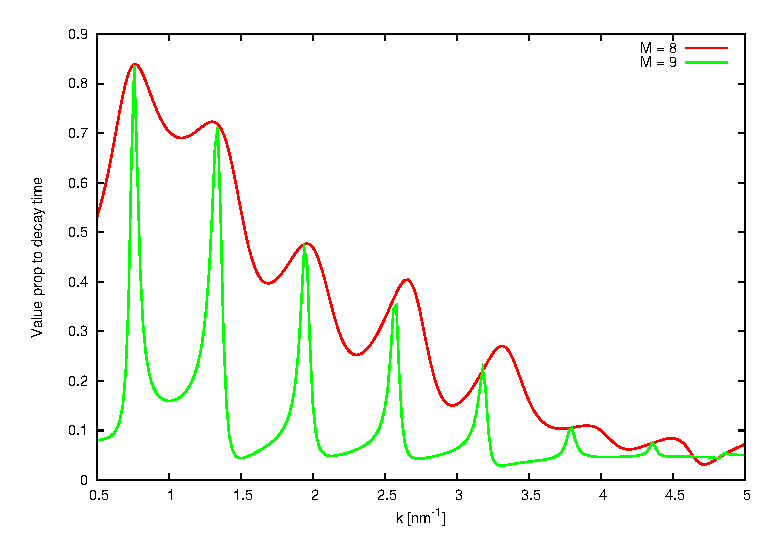
\includegraphics[]{tau.eps}
  \caption{The decay time against mode $k$.
  $k$ range is [0.5:0.01:5.0], $h_w=4.6$~nm.}
  \label{fig:tmp1}
\end{figure}


\end{document}